\documentclass[hide notes,red,handout]{beamer}
%\documentclass[handout,red,notes=show]{beamer}
% Class options include: notes, notesonly, handout, trans,
%                        hidesubsections, shadesubsections,
%                        inrow, blue, red, grey, brown

\usepackage{beamerthemesplit,soul,colortbl,color,multirow,fancybox, amsmath, amssymb, graphicx, dsfont, url,fancyhdr}
\usepackage[mathcal]{euscript}
\usepackage{booktabs}  % professionally typeset tables
\usepackage{textcomp}  % better copyright sign, among other things
\usepackage{xcolor}
\usepackage{lipsum,lscape}    % filler text
\usepackage{subfig}    % composite figures
\usepackage{tikz}


\setbeamersize{text margin left=0.6cm,text margin right=0.6cm}

\title{Overview of Statistical Learning}    % Enter your title between curly braces
\author{Justin Post}                 % Enter your name between curly braces
\date{September 5, 2014}                  % Enter the date or \today between curly braces

\begin{document}

% Creates title page of slide show using above information
\begin{frame}
  \titlepage
\end{frame}

\begin{frame}[t]
\frametitle{Statistical Learning}
A set of tools, procedure, and theory for modeling and understanding complex datasets.\\~\\
Encompasses
\begin{itemize}
\item Data mining - Finding patterns in datasets\\~\\
\item Inference - Determining which `inputs' (predictors) are associated with the 'output' (response)\\~\\
\item Prediction - Finding the best prediction method for an output based on a set of input variables
\end{itemize}
\end{frame}
\note{
It is a recently developed area in statistics and blends
with parallel developments in computer science and, in particular, machine
learning. The field encompasses many methods such as the lasso and sparse
regression, classification and regression trees, and boosting and support
vector machines.\\~\\
Data mining - patterns in data such as PC, Clustering, machine learning, regression (used often as an omnibus word)\\
Inference - learning where you care about the form of the model and the coefficients, not just the output (sometimes regression, etc.)\\
Prediction - form of the model not of interest, just best prediction possible.  Model averaging, bagging, boosting, etc.
}

\begin{frame}[t]
\frametitle{Two Major Situations for Learning}
\begin{itemize}
\item Learner - Model used\\~\\
\item Supervised Learning - Goal is to predict the value of an output (response) based on a number of inputs (predictors or features)\\~\\
\end{itemize}
\end{frame}

\begin{frame}[t]
\frametitle{Examples of Supervised Learning}
Supervised Learning - Goal is to predict the value of an output (response) based on a number of inputs (predictors or features)\\
\begin{itemize}
\item Multiple Linear Regression
$$Y_i = \beta_0+\beta_1x_{i1}+\beta_2x_{i2}+...+\beta_px_{ip}+E_i$$\pause
\item Ordinary Least Squares (OLS) estimates given in matrix form by 
$$\hat{\boldsymbol{\beta}}=(\boldsymbol{X}^{T}\boldsymbol{X})^{-1}\boldsymbol{X}^{T}\textbf{y}$$
where $\textbf{X}$ is called the `design matrix'
\end{itemize}
\[
\boldsymbol{X}=
\bordermatrix{~& & & & &\cr
~&1 & x_{11} & x_{12} &... &x_{1p} \cr
~&1 & x_{21} & x_{22} &... &x_{2p} \cr
~&\vdots & \vdots & \vdots &... &\vdots \cr
~&1 & x_{n1} & x_{n2} &... &x_{np}}
\]
\end{frame}

\begin{frame}[t]
\frametitle{Examples of Supervised Learning}
\begin{itemize}
\item Goal determines if `prediction' or `inference' is most important\\~\\
\item Possible model fitting procedures (other than OLS): \\\pause
\begin{itemize}
\item To improve prediction - Ridge Regression, Model Averaging, Neural Networks (Projection Pursuit Regression), ...\\~\\\pause
\item For better interpretation - LASSO, Elastic Net, Best Subset Regression, ...
\end{itemize}
\end{itemize}
\end{frame}

\begin{frame}[t]
\frametitle{Examples of Supervised Learning}
Economic survey of Pakistan over the years 1974-75 to 2000-01, yielding 28 observations (Pasha
and Akbar Ali Shah, 2004).\\~\\
Response = \# of persons employed (in millions)\\~\\\pause
Five predictors: \\
$x_1$ =land cultivated (in million hectors)\\
$x_2$ = inflation rate\\
$x_3$ = number of establishments\\
$x_4$ = population (in millions)\\
$x_5$ = literacy rate\\
\begin{itemize}\pause
\item Multiple Linear Regression
$$Y_i = \beta_0+\beta_1x_{i1}+\beta_2x_{i2}+\beta_2x_{i3}+\beta_2x_{i4}+\beta_5x_{i5}+E_i$$
\end{itemize}
\end{frame}

\begin{frame}[t]
\frametitle{Examples of Supervised Learning}
Note: OLS involves $(\boldsymbol{X}^{T}\boldsymbol{X})^{-1}$\\
\begin{center}
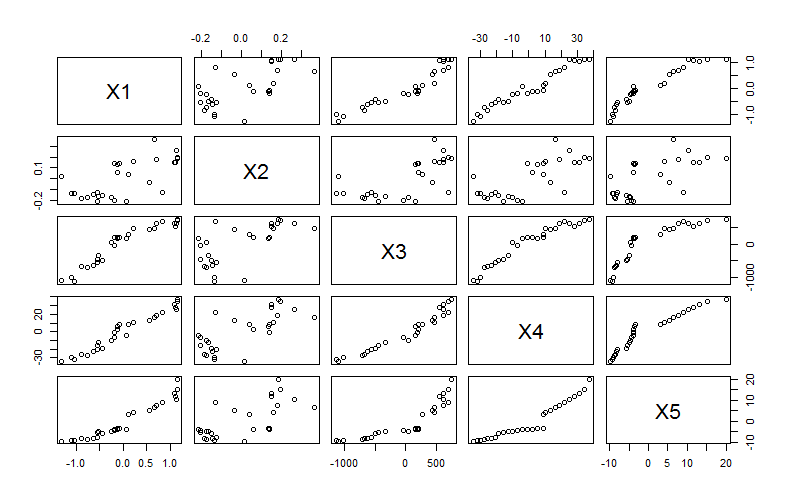
\includegraphics[scale=0.5]{scatters}
\end{center}
\end{frame}



\begin{frame}[t]
\frametitle{Examples of Supervised Learning}
Note: OLS involves $(\boldsymbol{X}^{T}\boldsymbol{X})^{-1}$\\~\\
\[
Cor(\boldsymbol{X})=
\bordermatrix{~&x_{1} & x_{2} &x_{3} &x_{4} &x_{5} \cr
&1 \cr
&0.664 &1 \cr
 & 0.943& 0.659& 1& \cr
& 0.976&0.729 &0.963 &1\cr
& 0.956 &0.681& 0.867& 0.951 &1\cr}.
\]~\\~\\\pause
$(\boldsymbol{X}^{T}\boldsymbol{X})^{-1}$ will be nearly singular! OLS estimates highly unstable.\\~\\
Ridge Regression can help stabilize estimates and increase prediction accuracy when predictors are correlated!  (We'll come back to this.)
\end{frame}

\begin{frame}[t]
\frametitle{Two Major Situations for Learning}
\begin{itemize}
\item Learner - Model used\\~\\
\item Supervised Learning - Goal is to predict the value of an output (response) based on a number of inputs (predictors or features)\\~\\
\item Unsupervised Learning - No outcome measure.  Goal is to describe the associations and patterns among a set of input measures.\\~\\
\end{itemize}
\end{frame}

\begin{frame}[t]
\frametitle{Example of Unsupervised Learning}
Unsupervised Learning - No outcome measure.  Goal is to describe the associations and patterns among a set of input measures.\\~\\
\begin{itemize}
\item Principal Components - Given $p$ inputs ($x_1,x_2,...,x_p$), attempt to find linear combinations that best 'represents' the data\\\pause
Find 
$$v_1=a_0x_1+a_1x_2+...+a_px_p=a^{T}\textbf{x}$$
so that $Var(a^{T}\textbf{x})$ is maximized.\\~\\\pause
Then find 
$$v_2=b_0x_1+b_1x_2+...+b_px_p=b^{T}\textbf{x}$$
so that $Var(b^{T}\textbf{x})$ is maximized subject to $v_1$ being orthogonal to $v_2$.\\~\\\pause
Repeat until `enough' of the variation in the $x's$ is described.
\end{itemize}
\end{frame}

\begin{frame}[t]
\frametitle{Example of Unsupervised Learning}
Using Pakistan economic data, we could find the principal components representation of the data.\\~\\
Since the data are very correlated, perhaps we can find a linear combination (or two) that accounts for most of the variation.\\~\\\pause
\begin{center}
\begin{tabular}{c|ccccc}
                    &      Comp.1 &    Comp.2  &   Comp.3   &   Comp.4    &   Comp.5\\
SD         & 2.093& 0.672& 0.366& 0.149& 0.100\\
Prop of Var& 0.876& 0.090& 0.027& 0.004& 0.002\\
Cum Prop   &0.876& 0.967& 0.994& 0.998& 1.000
\end{tabular}
\end{center}
First PC vector:
$$v_1=-0.467x_1 -0.375x_2 -0.456x_3 -0.474x_4 -0.458x_5 $$
\end{frame}

\begin{frame}[t]
\frametitle{Example of Unsupervised Learning}
Screeplot:
\begin{center}
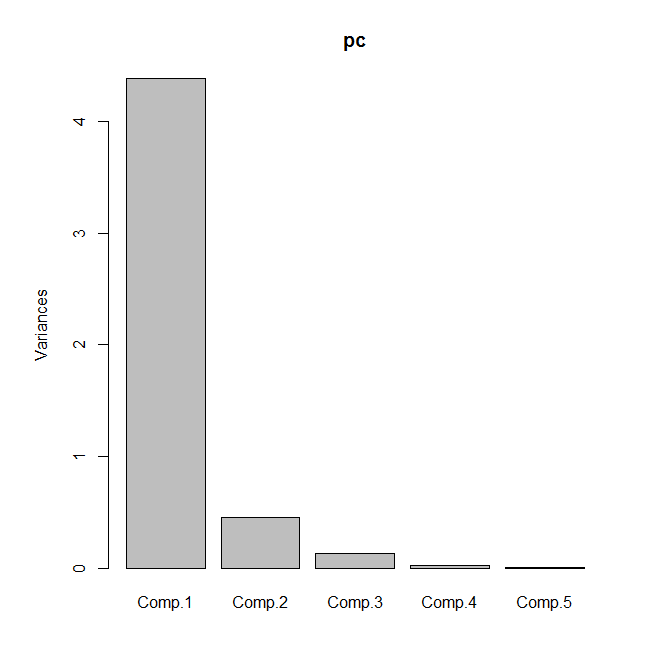
\includegraphics[scale=0.3]{screeplot}
\end{center}
First PC vector:
$$v_1=-0.467x_1 -0.375x_2 -0.456x_3 -0.474x_4 -0.458x_5 $$
\end{frame}


\begin{frame}[t]
\frametitle{Visualization of P.C.}
Consider just $x_1$ and $x_2$.  Below is a scatterplot with the PC directions plotted.
\begin{center}
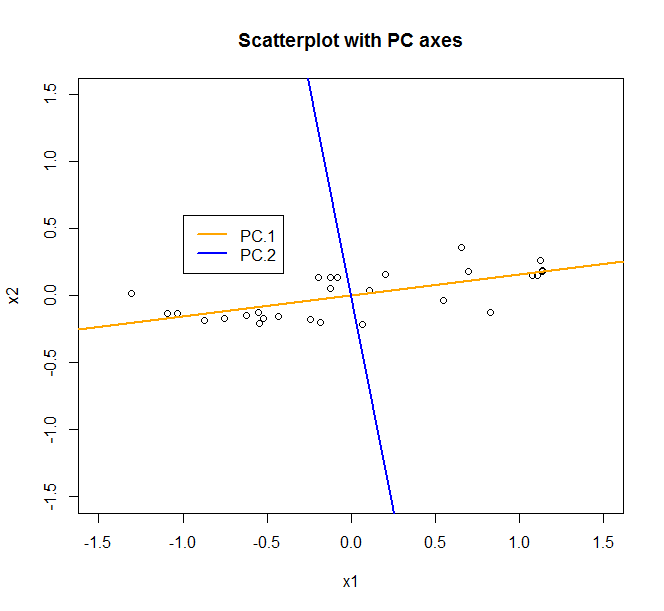
\includegraphics[scale=0.4]{pcvisualization}
\end{center}
\end{frame}



\begin{frame}[t]
\frametitle{Two Major Situations for Learning}
\begin{itemize}
\item Learner - Model used\\~\\
\item Supervised Learning - Goal is to predict the value of an output (response) based on a number of inputs (predictors or features)\\~\\
\item Unsupervised Learning - No outcome measure.  Goal is to describe the associations and patterns among a set of input measures.\\~\\
\begin{itemize}
\item Semi-supervised Learning - Some observations have an output variable, others do not
\end{itemize}
\end{itemize}
\end{frame}
%\note[enumerate]
%{\item Parameter greek vs statistic is latin 
%\item Describe general big idea of statistics with chart on board - idea of unbiased and random sample}

\begin{frame}[t]
\frametitle{Supervised Learning}
Readings: Most all of both Elements and Introduction cover Supervised Learning\\~\\\pause
Most problems can be classified as either
\begin{itemize}
\item Classification - output variable is categorical\\~\\
or \\~\\
\item Regression - output variable is quantitative\\~\\
\end{itemize}
Both can be viewed as a task in function approximation.
\end{frame}


\begin{frame}[t]
\frametitle{Selecting a Learner}
Consider having all quantitative inputs and output.\\~\\
Given values of $\textbf{X}$, we desire a function, $f(\textbf{X})$, for predicting $Y$.\\~\\\pause
Also require a `Loss function' for determining adequacy of fit, $L(Y,f(\textbf{X}))$.\\~\\
Most commonly used Loss function is squared error
$$L(Y,f(\textbf{X}))=(Y-f(\textbf{X}))^2$$\pause
Now, criterion for selecting $f()$ is to minimize expected loss.
$$E\left[(Y-f(\textbf{X}))^2\right]$$
\end{frame}

\begin{frame}[t]
\frametitle{Selecting a Learner}
Often a good choice for $f()$ is $E(Y|X=x)$. \\~\\
This is the solution for Linear Regression:
$$\hat{y}=E(Y|X=x)=\hat{\beta_0}+\hat{\beta_1}x_1+...+\hat{\beta_p}x_p$$~\\
A simple solution that works in many situations.\\~\\\pause
However, when selecting a model there is a constant trade-off between the bias in the model and the variability of the prediction (estimates).
\end{frame}


\begin{frame}[t]
\frametitle{Bias/Variance Trade-off}
Linear model, $f(\textbf{X})\approx\textbf{X}^T\beta$, often has low variance but possibly high bias wrt $f$.\\~\\
Consider classifying a binary response (0,1) with 2 quantitative pred's.
\begin{center}
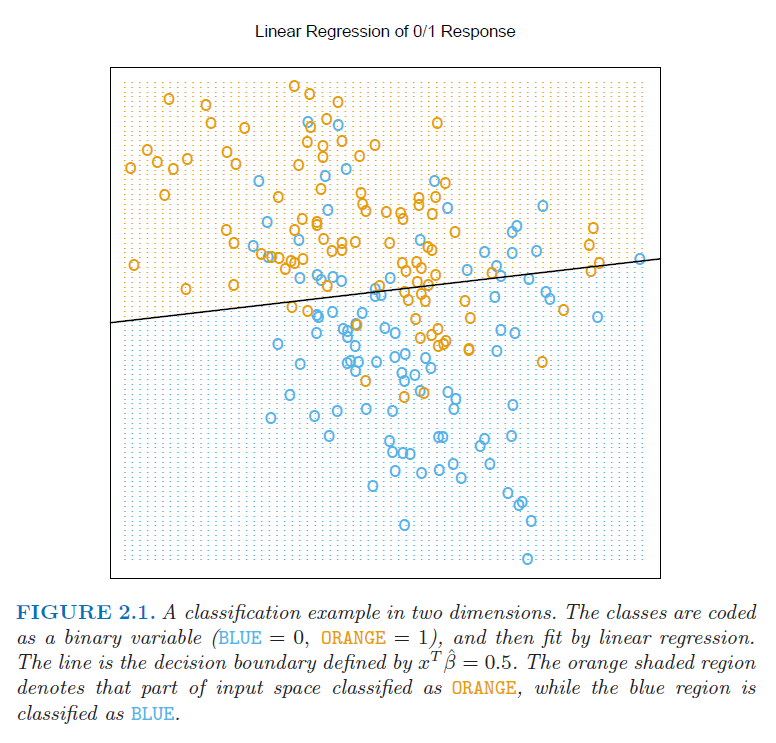
\includegraphics[scale=0.3]{biasslr}
\end{center}
\end{frame}
\note{High Variance - new data set, likely to get vastly different answers.\\
High Bias - Linearity restriction may lead to poor prediction for some values.}

\begin{frame}[t]
\frametitle{Bias/Variance Trade-off}
Using a local method, such as `k-nearest neighbors' (knn) has low bias but high variance.\\~\\\pause
\begin{itemize}
\item Use $k$ 'closest' (judged by say, Euclidean distance) values to determine classification (0 or 1).  \\~\\
\item If knn have proportion of 1's greater than 0.5, assign 1.\\~\\
\item If knn have proportion of 1's less than or equal to 0.5, assign 0.
\end{itemize}
\end{frame}

\begin{frame}[t]
\frametitle{Bias/Variance Trade-off}
\begin{center}
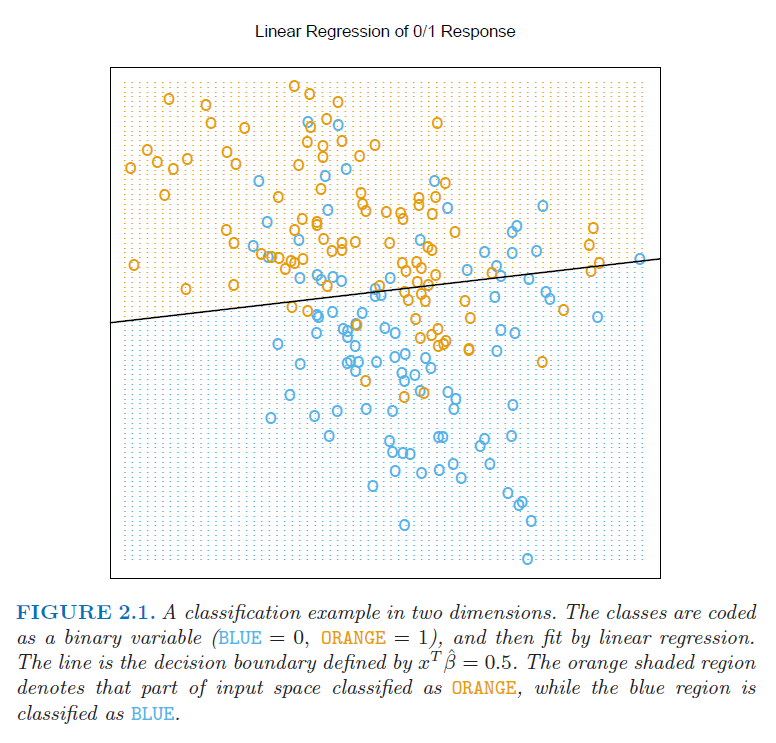
\includegraphics[scale=0.27]{biasslr}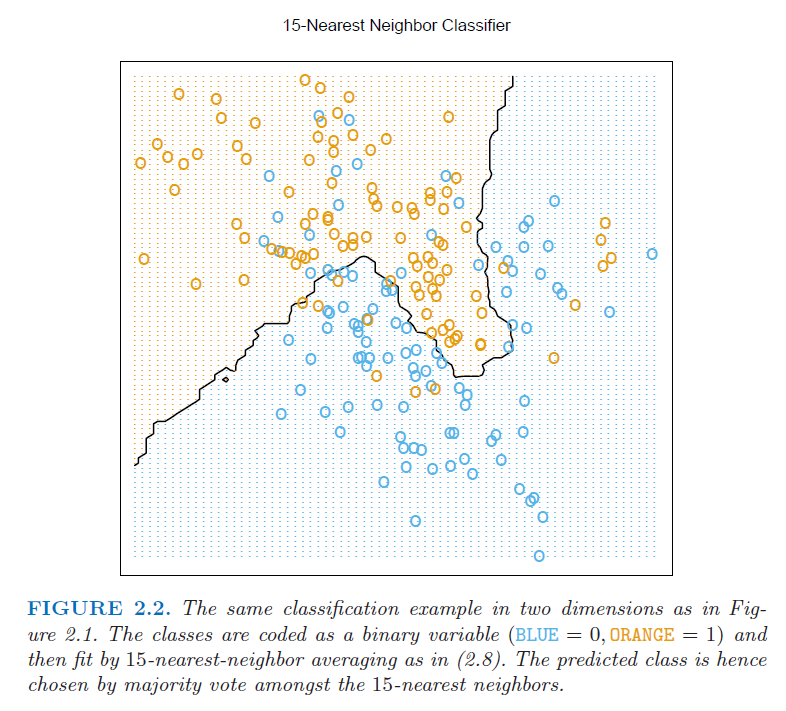
\includegraphics[scale=0.27]{knn}
\end{center}
\end{frame}


\begin{frame}[t]
\frametitle{General Methods for choosing $f()$}
Parametric - Assume a form for $f()$ leaving us estimation of the resulting parameters \\~\\\pause
\begin{enumerate}
\item Make an assumption about function form.  Ex:
$$f(X)=\beta_0+\beta_1 x_1+...+\beta_p x_p$$\pause
\item Find parameter estimates by minimizing expected loss.  Since we can't actually do this we minimize observed loss.  Ex:
$$min_{\beta's}\sum_{i=1}^{n}(y_i-\beta_0-\beta_1x_{i1}-...-\beta_px_{ip})^2$$~\\
\end{enumerate}
Main drawback, functional form may be incorrect!
\end{frame} 


\begin{frame}[t]
\frametitle{General Methods for choosing $f()$}
Non-Parametric - No functional form chosen, but put constraint on the `wiggly-ness' of the function.\\\pause
\begin{itemize}
\item Can lead to better `fit' as a wide variety of $f$'s can be used.\\~\\
\item Problem difficult as $f$ can be complicated\\~\\
\item Need many observations!\\~\\\pause
\end{itemize}
Curse of Dimensionality - Any method that attempts to produce locally varying functions in small neighborhoods will run into problems in high dimensions as `local' becomes prohibitively big.
\end{frame}

\begin{frame}[t]
\frametitle{Ridge Regression Example}
Pakistan example -\\~\\
\begin{itemize}
\item Assume linear model is true $f$.  MLR model in which errors have mean zero and are uncorrelated with constant variance. \\~\\
\item $\rightarrow$ OLS is 'best' (smallest variance) linear unbiased estimates (by Gauss-Markov Theorem).\\~\\\pause
\item $X_1$-$X_5$ highly correlated.  Leads to high variance of estimates.\\~\\\pause
\item Perhaps we can get a better model by trading having a little bias, but less variance.\\~\\
\item RR increases bias but decreases variance .
\end{itemize}
\end{frame}


\begin{frame}[t]
\frametitle{Ridge Regression Example}
RR estimates minimize a penalized loss function:
$$min_{\beta}\sum_{i=1}^{n}(y_i-\beta_0-\beta_1x_{i1}-...-\beta_px_{ip})^2+\lambda\sum_{i=1}^{n}\beta_i^2$$
or
$$\hat{\boldsymbol{\beta}}_{RR}=min_{\boldsymbol{\beta}}||\boldsymbol{y}-\boldsymbol{X}\boldsymbol{\beta}||^2+\lambda\boldsymbol{\beta}^{T}\boldsymbol{\beta}$$
where $\lambda$ is a `tuning parameter.'\\~\\\pause
If $\lambda$=0, then there is no penalty and you get the usual OLS solution.\\~\\
If $\lambda$ is big, then $\beta$ values that minimize this will be `shrunk'.
\end{frame}

\begin{frame}[t]
\frametitle{Ridge Regression Example}
RR solution has nice matrix form
$$\hat{\boldsymbol{\beta}}_{RR}=(\boldsymbol{X}^{T}\boldsymbol{X}+\lambda \boldsymbol{I}_{p})^{-1}\boldsymbol{X}^{T}\boldsymbol{y}$$
\begin{center}
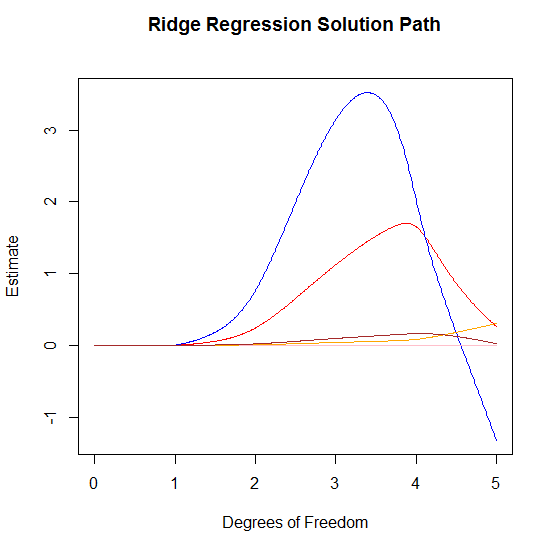
\includegraphics[scale=0.4]{rrpath}
\end{center}
\end{frame}



\begin{frame}[t]
\frametitle{Principal Components and Ridge Regression}
\begin{itemize}
\item Principal component with the smallest variance has its coordinates shrunk more.	\pause
\item This can be seen using the predicted values:
$$\hat{\boldsymbol{y}}=\boldsymbol{X}\hat{\boldsymbol{\beta}}_{RR} = \boldsymbol{X}(\boldsymbol{X}^{T}\boldsymbol{X}+\lambda \boldsymbol{I}_{p})^{-1}\boldsymbol{X}^{T}\boldsymbol{y}$$
Using the SVD of $\boldsymbol{X}$
$$\boldsymbol{X}^{T}\boldsymbol{X}=(\boldsymbol{U}\boldsymbol{D}\boldsymbol{V}^{T})^{T}(\boldsymbol{U}\boldsymbol{D}\boldsymbol{V}^{T})=\boldsymbol{V}\boldsymbol{D}^2\boldsymbol{V}^{T}$$\pause
We now have
$$\hat{\boldsymbol{y}}=\boldsymbol{U}\boldsymbol{D}(\boldsymbol{D}^2+\lambda\boldsymbol{I}_p)^{-1}\boldsymbol{D}\boldsymbol{U}^{T}\boldsymbol{y}$$
$$=\sum_{j=1}^{p}\boldsymbol{u}_j\frac{d_j^2}{d_j^2+\lambda}\boldsymbol{u}_{j}^{T}\boldsymbol{y}$$
$d_j$ is the $j^{th}$ eigenvalue and $\boldsymbol{u}_{j}$ is the $j^{th}$ normalized prin comp of $\boldsymbol{X}$.
\end{itemize}
\end{frame}


\begin{frame}[t]
\frametitle{Principal Components Regression}
\begin{itemize}
\item Principal component regression is an alternative to shrinking all eigenvectors some.\\~\\\pause
\item Here, shrink the smallest eigenvectors to 0 and leave the largest ones untouched.\\~\\
\item That is, simply conduct a regression using the `most important' eigenvectors as your predictors.
$$Y_i=\beta_0+\beta_1v_{i1}+...\beta_kv_{ik}+E_i$$
where $k\leq p$.
\end{itemize}
\end{frame}



\begin{frame}[t]
\frametitle{Upcoming Reading Group Topics}
\begin{itemize}
\item September 19, Brian Gaines - Overview of Regularization Methods\\
\begin{itemize}
\item Following 2 weeks' topics will be more in depth on Regularization\\~\\\pause
\end{itemize}
\item October 17, Neal Grantham - Overview of Classification Methods\\
\begin{itemize}
\item Following 2 weeks' topics will be more in depth on Classification\\~\\\pause
\end{itemize}
\item November 7, Jami Jackson - Overview of Support Vector Machines\\
\begin{itemize}
\item Following 2 weeks' topics will be more in depth on SVM
\end{itemize}
\end{itemize}
\end{frame}

\begin{frame}[t]
\frametitle{Stat Faculty working in Statistical Learning}
\begin{itemize}
\item Hua Zhou\\~\\
\item Eric Laber\\~\\
\item Rui Song\\~\\
\item Jessie Jeng\\~\\
\item Yichao Wu\\~\\
\item Howard Bondell\\~\\
\item Dave Dickey\\~\\
\item Wenbin Lu\\~\\
\end{itemize}
\end{frame}


\end{document} 

